\documentclass[12pt]{extarticle}

\usepackage[letterpaper,margin=0.35in]{geometry}
\usepackage[T1]{fontenc}
\usepackage[scaled=0.95]{helvet}
\renewcommand{\familydefault}{\sfdefault}
\usepackage{microtype}
\usepackage[table]{xcolor}
\usepackage{graphicx}
\usepackage{tabularx}
\usepackage{array}
\usepackage{booktabs}
\usepackage{enumitem}
\usepackage[most]{tcolorbox}
\usepackage{setspace}

\definecolor{agencyblue}{HTML}{005A8B}
\definecolor{deepsea}{HTML}{143B5D}
\definecolor{labline}{HTML}{A9BBC8}
\definecolor{panelbg}{HTML}{F6F8FA}
\definecolor{titlebg}{HTML}{EAF2F7}
\definecolor{textgray}{HTML}{2F3B45}

\pagecolor{white}
\pagestyle{empty}
\color{textgray}
\setstretch{0.92}
\setlength{\parindent}{0pt}
\setlength{\parskip}{0pt}
\setlength{\tabcolsep}{3pt}
\renewcommand{\arraystretch}{1.02}
\setlist[itemize]{leftmargin=1.0em,labelsep=0.35em,itemsep=0.4pt,topsep=0.8pt,parsep=0pt}
\setlist[enumerate]{leftmargin=1.1em,labelsep=0.35em,itemsep=0.4pt,topsep=0.8pt,parsep=0pt}
\newcolumntype{Y}{>{\raggedright\arraybackslash}X}
\hyphenpenalty=10000
\exhyphenpenalty=10000
\tolerance=2000
\emergencystretch=8pt

\newtcolorbox{labbox}[2][]{
  colback=panelbg,
  colframe=labline,
  colbacktitle=titlebg,
  coltitle=deepsea,
  fonttitle=\bfseries\small,
  title=\MakeUppercase{#2},
  boxrule=0.5pt,
  arc=0pt,
  left=4pt,
  right=4pt,
  top=2pt,
  bottom=2pt,
  toptitle=1pt,
  bottomtitle=1pt,
  #1
}

\begin{document}
\footnotesize

\begin{tcolorbox}[
  colback=white,
  colframe=deepsea,
  boxrule=0.9pt,
  arc=0pt,
  left=7pt,
  right=7pt,
  top=5pt,
  bottom=4pt
]
\begin{minipage}[c]{0.14\textwidth}
\centering
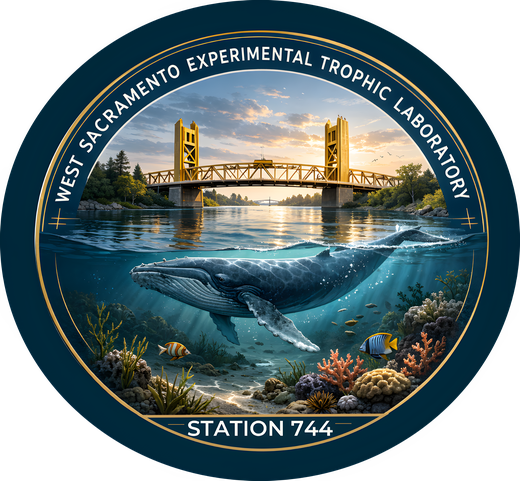
\includegraphics[width=\linewidth]{../images/logo_small.png}
\end{minipage}\hfill
\begin{minipage}[c]{0.82\textwidth}
{\scriptsize\textbf{\color{agencyblue}W.E.T. LAB FIELD OPERATIONS UNIT}}\par
\vspace{3pt}
{\Large\bfseries\color{deepsea}Player Briefing: How To Play}\par
\vspace{4pt}
{\small Team science party game | Mini-games, hidden funding, lightning talks, and one squid problem}
\end{minipage}

\vspace{3pt}
{\footnotesize
\rowcolors{1}{titlebg}{white}
\begin{tabularx}{\textwidth}{@{}>{\bfseries\color{deepsea}}l Y >{\bfseries\color{deepsea}}l Y@{}}
Objective & Finish with the most total funding & Team size & 4-5 players per lab \\
Core phases & Compete, prepare proposal, give lightning talk, resolve squid theft & Currency & All values are in \$100 increments \\
\end{tabularx}}
\end{tcolorbox}

\vspace{2pt}

\begin{minipage}[t]{0.492\textwidth}
\vspace{0pt}
\begin{labbox}{Win Condition}
Finish with the \textbf{highest total funding}. Money comes from:
\begin{itemize}
\item winning mini-games
\item earning \textbf{+\$100} for completing all mini-games
\item finding hidden \$100 discoveries
\item earning proposal awards during lightning talks
\end{itemize}
\end{labbox}

\begin{labbox}{Game Flow}
\begin{enumerate}
\item Get your identity badge and role.
\item Form labs of 4-5 players.
\item Play head-to-head station games during the game phase.
\item Record all results in your lab notebook.
\item Prepare a research pitch under 2 minutes.
\item Give your lightning talk and receive peer-review funding.
\item Resolve squid theft, then total funding.
\end{enumerate}
\end{labbox}

\begin{labbox}{Team Rules}
\begin{itemize}
\item Teams of 4 receive \textbf{+\$150}.
\item Teams lock after formation unless the host changes them.
\item Keep one lab notebook for wins and discoveries.
\item \textbf{Mini-game wins need an opposing signature} to count.
\item Completing every mini-game earns the lab \textbf{+\$100}.
\end{itemize}
\end{labbox}

\begin{labbox}{Your Role May Matter}
\scriptsize
\begin{tabularx}{\linewidth}{@{}>{\bfseries}p{0.27\linewidth}Y@{}}
Data Scientist & May call \textbf{Model Overfit} before one mini-game; that game's winner gets double funding. \\
Geneticist & Create \textbf{one hybrid organism}; it counts as both species for the rest of the game. \\
Oceanographer & Gets \textbf{3 clues} to hidden \$100 discoveries and may search during play. \\
Dolphin & Must be the dolphin in \textbf{Dolphin Trainer}. \\
Whale & Your lab gains \textbf{+\$200} per whale. \\
Squid & After scoring, may steal \textbf{\$200} from one rival team. \\
\end{tabularx}
\end{labbox}

\begin{labbox}{Proposal And Review}
\begin{itemize}
\item After station play, your lab gets ~ \textbf{15 minutes} to build a research pitch.
\item Lightning talk limit: \textbf{under 2 minutes}.
\item \textbf{Peer reviewers} should remain anonymous until after scoring.
\item Reviewers \textbf{cannot score their own team}.
\end{itemize}

\vspace{2pt}
\begin{tabularx}{\linewidth}{@{}Y >{\raggedleft\arraybackslash}p{0.16\linewidth}@{}}
\toprule
Proposal award & Value \\
\midrule
Most Scientifically Plausible & \$400 \\
Best Delivery & \$300 \\
Funniest & \$200 \\
\bottomrule
\end{tabularx}
\end{labbox}
\end{minipage}\hfill
\begin{minipage}[t]{0.492\textwidth}
\vspace{0pt}
\begin{labbox}{Mini-Game Phase}
Games are \textbf{team vs. team}. Use the station instructions and record awards immediately.

\vspace{2pt}
If your lab completes all mini-games, add a \textbf{+\$100 completion bonus}.

\vspace{2pt}
\begin{tabularx}{\linewidth}{@{}Y >{\raggedleft\arraybackslash}p{0.16\linewidth}@{}}
\toprule
Station & Award \\
\midrule
Plankton Survival & \$200 \\
Marine Mammal Relay & \$300 \\
Baleen Simulator & \$200 \\
Dolphin Trainer & \$300 \\
Fish Bowl & \$300 \\
Snorkel Soccer & \$200 \\
Specimen Catalog & \$250 \\
Competitive Feeding & \$200 \\
\bottomrule
\end{tabularx}
\end{labbox}

\begin{labbox}{Endgame}
\begin{enumerate}
\item Add mini-game funding, the \textbf{+\$100} all-mini-games bonus if earned, hidden cash, whale prestige, and proposal awards.
\item Then each squid may steal \textbf{\$200} from one rival team.
\item Recalculate totals after all squid theft is resolved.
\item Highest final funding total wins.
\end{enumerate}
\end{labbox}

\begin{labbox}{Tips}
\begin{itemize}
\item Chase easy station wins early.
\item Do not ignore the proposal round.
\end{itemize}
\end{labbox}

\end{minipage}

\vfill
\begin{center}
\footnotesize\color{agencyblue}\textbf{W.E.T. LAB | Player Quick Reference | Internal Use Only}
\end{center}

\end{document}
